% !TeX program = pdflatex
% Supplementary Information, unified rewrite 2026-11-12.
% Every number resolves to master_unified_v1.csv (profile_v1 extraction)
% or to the frozen verdict and audit tables cited in the text.
\documentclass[11pt,a4paper]{article}

\usepackage[T1]{fontenc}
\usepackage[utf8]{inputenc}
\usepackage{lmodern}
\usepackage[margin=2.2cm]{geometry}
\usepackage{amsmath,amssymb}
\usepackage{booktabs}
\usepackage{array}
\usepackage{longtable}
\usepackage{placeins}
\usepackage{graphicx}
\graphicspath{{figs/}}
\usepackage[colorlinks=true,linkcolor=blue,citecolor=blue,urlcolor=blue]{hyperref}
\usepackage{microtype}

\renewcommand{\thesection}{S\arabic{section}}
\renewcommand{\thesubsection}{\thesection.\arabic{subsection}}
\renewcommand{\thetable}{S\arabic{table}}
\renewcommand{\thefigure}{S\arabic{figure}}

\setlength{\tabcolsep}{4pt}
\setlength{\parindent}{0pt}
\setlength{\parskip}{4pt}

\title{\bfseries Supplementary Information\\[4pt]
\large Gating time constants are the conserved coordinates of cardiac ion
channels: a unified reanalysis of seven voltage-clamp corpora}
\author{Huan Li}
\date{}

\begin{document}
\maketitle

\noindent This document contains the identifiability analysis of the
thirteen-parameter hERG formulation (S1), the per-corpus extraction methods
(S2), the robustness calibres of the conservation verdict (S3), the
five-laboratory CiPA dataset methods with its official-table defects and defect
registry (S4), the reasons Kir and K2P channels do not enter the verdict (S5),
the per-group verdict table (S6), the host-model integration and CiPA scoring
details (S7) and the data and code deposition (S8). Every number in the main
text resolves to a table here or to the deposited master table.

\tableofcontents
\newpage

\section{Identifiability of the thirteen-parameter hERG formulation}

The thirteen-parameter hERG scheme is a four-state Markov ring with a
double-exponential activation edge, a parallel slow component and a per-cell
conductance. It was calibrated on the four protocol families of the
construction cell (steady activation, deactivation staircase, sinusoidal wave,
action-potential clamp) and passes seven of eight pre-set criteria. The Fisher
matrix of Eq.~(1) of the main text was assembled by central finite differences
($10^{-3}$\,dex steps for log-scaled parameters, $10^{-3}|pf_2|$ for the one
linear parameter) on an independent expm simulation channel, weighted by
per-segment residual variance. Automatic differentiation was not used; the
finite-difference construction is the one whose results are reported.

\begin{table}[htbp]\centering\small
\caption{Fisher eigenvalues in ascending order ($\lambda_{\max}=2.29228\times10^{9}$;
condition number $7.3798\times10^{12}$; span 12.87 orders of magnitude).}
\begin{tabular}{@{}cl@{}}
\toprule
index & eigenvalue \\
\midrule
1 & $3.10618\times10^{-4}$ \\
2 & $3.14380\times10^{4}$ \\
3 & $1.59570\times10^{5}$ \\
4 & $4.10533\times10^{5}$ \\
5 & $9.83394\times10^{5}$ \\
6 & $1.37507\times10^{6}$ \\
7 & $2.40444\times10^{6}$ \\
8 & $3.30837\times10^{6}$ \\
9 & $8.69487\times10^{6}$ \\
10 & $5.70476\times10^{7}$ \\
11 & $1.57368\times10^{8}$ \\
12 & $2.68717\times10^{8}$ \\
13 & $2.29228\times10^{9}$ \\
\bottomrule
\end{tabular}
\end{table}

Null directions are defined as eigenvalues below $10^{-3}$ of the largest
($2.29228\times10^{6}$). The count of six is a convention: the sixth eigenvalue
sits at $6.0\times10^{-4}$ of the largest and the seventh at
$1.05\times10^{-3}$, on either side of the cut.

\begin{table}[htbp]\centering\small
\caption{Null directions below $10^{-3}\lambda_{\max}=2.29228\times10^{6}$.}
\begin{tabular}{@{}clp{4.2cm}p{5.2cm}@{}}
\toprule
\# & $\lambda$ & dominant parameters & interpretation \\
\midrule
0 & $3.1\times10^{-4}$ & $\log_{10}P_1$, $\log_{10}P_{f1}$, $\log_{10}P_2$ & activation double-exponential amplitude--component compensation (near-exact null) \\
1 & $3.1\times10^{4}$ & $\log_{10}P_2$, $\log_{10}P_{f2}$ & voltage-dependence coefficients of the two exponentials compensate \\
2 & $1.6\times10^{5}$ & $\log_{10}\alpha_\tau$, $\log_{10}\alpha_{\mathrm{amp}}$, $\log_{10}P_3$ & slow-component time constant and amplitude compensate \\
3 & $4.1\times10^{5}$ & $\log_{10}P_7$, $\log_{10}P_5$, $\log_{10}P_6$ & inactivation--recovery edges compensate \\
4 & $9.8\times10^{5}$ & $\log_{10}\alpha_{\mathrm{amp}}$, $\log_{10}P_3$, $\log_{10}\alpha_\tau$ & slow amplitude and $k_{34}$ share the rebound peak \\
5 & $1.4\times10^{6}$ & $\log_{10}P_3$, $\log_{10}\alpha_{\mathrm{amp}}$, $\log_{10}G_{\mathrm{Kr}}$ & absolute-scale triad \\
\bottomrule
\end{tabular}
\end{table}

One degeneracy is exact rather than numerical. With the maximum open
probability frozen, the combination
$\alpha_{\mathrm{amp}}\cdot\mathrm{ALPHA}\cdot\mathrm{XMAX}$ enters the
likelihood only as a product, so no experiment can separate its factors. A
second degeneracy is near-exact: exchanging the two exponential components of
the activation edge costs
$\lambda/\lambda_{\max}\approx1.4\times10^{-13}$.

The joint rate--conductance rescaling usually assumed in this literature is
not a degeneracy of the fitted model. Rescaling all rates by $s$ and the
conductance by $1/s$ maps $I(V,t)$ to $s^{-1}I(V,st)$, which differs from
$I(V,t)$ on any fixed protocol time grid. Table~\ref{tab:rescale} quantifies
the break: the data already reject a 1\% rescaling, and a 10\% rescaling moves
the predicted waveform by 18--45\% depending on protocol.

\begin{table}[htbp]\centering\small
\caption{Rate--conductance joint rescaling: relative waveform change
$\Delta_s$ for the four protocol families. The pre-set criterion was
$\Delta<0.01$ (approximately degenerate) and $\Delta>0.05$ (broken) at
$s=1.1$; the data break the rescaling already at $s=1.01$.}
\label{tab:rescale}
\begin{tabular}{@{}lccccc@{}}
\toprule
protocol & $s=1.01$ & $s=1.05$ & $s=1.1$ & $s=1.5$ & $s=2.0$ \\
\midrule
steady activation & 0.0233 & 0.1049 & 0.1826 & 0.3796 & 0.7555 \\
deactivation & 0.0258 & 0.1235 & 0.2334 & 0.7587 & 0.9498 \\
sine wave & 0.0553 & 0.2537 & 0.4517 & 0.9614 & 1.2308 \\
action potential & 0.0338 & 0.1559 & 0.2831 & 0.7486 & 1.0901 \\
\bottomrule
\end{tabular}
\end{table}

The serial-state variant, in which extra closed states are added to repair the
peak--sine exclusion, passes all eight criteria but is not identifiable: the
Cram\'er--Rao bounds on its rate multipliers are $\pm9.6$--$13.2$\,dex against
a data-supported window of $\pm0.017$\,dex, a factor of about 760.

\FloatBarrier
\section{Per-corpus extraction methods}

All corpora share one schema and one interval construction (per-row 95\%
profile likelihood, nuisance parameters refit on a grid over the target,
$F$-statistic threshold). What differs per corpus is the segmentation, the fit
windows and the quality-control chain, summarised here.

\subsection{Channelpedia}

Automated patch-clamp NWB files with per-cell JSON metadata; 19,282 cells
downloaded, 17,987 retained after quality control. Activation, deactivation,
inactivation and recovery segments were fit per sweep with mono- or
bi-exponential decays (component count fixed per channel family), steady-state
curves by Boltzmann fits. Recordings at 15, 25 and 35\,$^\circ$C were used.
Groups with fewer than 15 cells do not enter a verdict. Rows whose fit reaches
a window or bound are flagged \texttt{tau\_edge} and retained. Kv1.5 at
15\,$^\circ$C and the K2P rows carry this flag most often.

\subsection{CiPA five-laboratory hERG}

Manual patch-clamp per-cell waveforms (62\,GB, 14{,}973 csv files,
sha256-verified) of 28 drugs under the standardised ICH S7B Q\&A 2.1 protocol
with blinded replicate arms. Sweep metadata exist for only two directory
trees, so vehicle, drug-block and steady-state windows were segmented from the
waveform plateaus alone and the segmentation was then validated against the
two metadata-carrying directories. Tail deactivation time constants were
extracted per sweep with profile intervals. The per-cell ratio references the
steady-state (highest-concentration) window to the vehicle window of the same
cell. Of 1,875 cells passing trace-level quality control, 1,750 contribute
deactivation windows to the master table and 970 have both segments valid for
the ratio. Current-unit suffixes differ across laboratories and were read from
the column names (laboratory 2 records amperes, the others pA; the conversion
map is part of the frozen pipeline). Voltage-contaminated current columns in
three laboratories were detected by a corrupted-column screen and excluded.
Defects are registered in S4.

\subsection{Lei five-temperature hERG series}

Automated recordings of hERG at 25, 27, 31, 35 and 37\,$^\circ$C (670 wells).
Recovery, fast activation and fast deactivation time constants were extracted
per well with profile intervals. The 27\,$^\circ$C recovery batch carries
batch noise (a slow tail around 3.2\,s), so the temperature law of the main
text is stated on the recovery component, which is monotone across the five
temperatures.

\subsection{Beattie nine-cell manual hERG dataset}

Nine cells, six protocols, manual patch at 37\,$^\circ$C. Steady-state
activation was measured by the tail-current method rather than the
holding-segment mean; the tail method removes a Boltzmann degeneracy that
otherwise pushes midpoint fits to their bounds. Deactivation was fit with two
exponential components per sweep.

\subsection{Na\textsubscript{v}1.5 two-temperature series}

Whole-cell Nav1.5 recordings at 25 and 35\,$^\circ$C under five compound
levels (four cells). Inactivation time constants were measured from
peak-aligned decay windows at 40\,\textmu s sampling. Rows reaching the
9\,ms fit ceiling at 25\,$^\circ$C are flagged \texttt{tau\_edge}.

\subsection{Ca\textsubscript{v}1.2 pharmacology dataset}

Six cells with Ca$^{2+}$ and Ba$^{2+}$ charge carriers and a continuous
bath-temperature channel recorded alongside every sweep; temperature therefore
enters as a measured covariate, not a nominal label. Calcium-dependent
inactivation time constants were extracted per sweep. Inactivation under
Ba$^{2+}$ is too slow for the 180\,ms window; those rows carry the
\texttt{tau\_edge} flag and are excluded from time-constant statistics but
retained in the table.

\subsection{I\textsubscript{Ks} activation series}

283 recordings of KCNQ1/KCNE1. Activation delay and time constant were fit
jointly on the step epoch; deactivation time constants come from the
$-40$\,mV tail epoch. Duplicate recordings of the same cell were resolved to
the single best-quality version before fitting.

\subsection{Reference layers}

Three reference layers are stored in the master-table schema: official CiPA
potency anchors (IC$_{50}$ and Hill coefficients, 29 drugs across seven
channels, 250 rows), cross-species group comparisons (38 pairs, 76 rows), and
ten gating-layer summaries of 933 deduplicated published models from
ICGenealogy whose gating curves were refit in-house (30 rows).

\FloatBarrier
\section{Robustness of the conservation verdict}

The headline calibre (D) estimates the group-level true scatter by
hierarchical partial pooling with marginal likelihood, propagating per-row
profile-likelihood uncertainties (asymmetric half-widths averaged). Three
other calibres bracket it: (A) the raw across-cell scatter ratio with no
shrinkage; (B) calibre A after removing Boltzmann midpoint fits that hit their
voltage bounds; (C) two-stage hierarchical shrinkage with symmetric standard
errors. Table~\ref{tab:calibres} gives the Kv-activation verdict under all
four.

\begin{table}[htbp]\centering\small
\caption{The Kv-activation verdict under four calibres (64 groups). Calibres
differ only in how scatter and uncertainty are estimated; the verdict is
unchanged.}
\label{tab:calibres}
\begin{tabular}{@{}p{6.2cm}cc@{}}
\toprule
calibre & pass & median ratio \\
\midrule
A: raw observed scatter & 63/64 & 3.37 \\
B: bound-hit midpoints removed & 63/64 & 2.87 \\
C: hierarchical shrinkage, symmetric errors & 63/64 & 2.48 \\
D: C with profile-likelihood intervals (headline) & 63/64 & 2.48 \\
\bottomrule
\end{tabular}
\end{table}

Across all 194 evaluable groups of the five verdict tables, moving from
calibre C to calibre D changes exactly one verdict: Kv1.7 recovery at
15\,$^\circ$C moves from 1.009 to 0.995, sitting on the threshold in both
calibres. The hierarchical time-constant estimates differ from the unshrunk
values by a median of $-1.3\%$ per group, so the scatter estimates are nearly
unbiased. The 66-group frame of earlier drafts contained two TASK-3 groups;
K2P leak channels have no sigmoidal gating and their inclusion was registered
as a grouping impurity, giving the 64-group activation frame used here.

\FloatBarrier
\section{CiPA five-laboratory dataset: results, official-table defects and registry}
\label{sec:fivelab}

\subsection{Central results on the new extraction}

The drug-versus-vehicle deactivation $\tau$ ratio, referenced within cell to
the steady-state highest-concentration block window, has pooled median 0.948
($n=970$ cells; 43.3\% of cells inside the 0.80--1.25 band, 55.4\% within
$\pm30\%$). Per-laboratory medians are 1.05, 0.99, 0.81, 0.92 and 1.17
(laboratories 1--5). The laboratory-3 value, a 19\% acceleration, is the
largest deviation in the dataset. Stratum medians by steady-state block
fraction run 0.96, 0.90, 0.89, 1.01 and 1.07 from shallow to deep block: the
ratio does not drift with occupancy. The blinded arm reproduces the unblinded
one through the same frozen pipeline (medians 0.87 on $n=102$ blinded cells
against 0.96 on $n=868$ unblinded). Our per-drug IC$_{50}$ estimates match the
official CiPA values within ten-fold for 23 of 24 drugs.

\subsection{Earlier frozen audit stages carried forward}

The following dataset-level findings of the frozen audit are independent of
the extraction-calibre change and are carried forward unchanged.
Cross-laboratory IC$_{50}$ fold differences have median 6.17 over 28 drugs,
consistent with the source study's reported natural variability of roughly
five-fold. Laboratory 2 is systematically high by 3.10-fold and the shift
localises to the addition method: it disappears (0.77) when that laboratory
assays real experimental samples. A leak-current explanation was excluded:
within-laboratory correlation between holding leak and block is null
(laboratory 2, Spearman $\rho=+0.006$, $n=441$) and the block fraction is
computed on a peak-minus-baseline difference, which cancels any constant leak
residual. State-dependent binding is visible in three independent waveform
signatures: Hill coefficients differ from one in 42 of 134 drug-laboratory
sets; the peak-to-plateau shape ratio under deep block is 0.73 in laboratory
1; and 36--39\% of first/second exposure segments end before block plateaus.
The apparent on-rate of block is flattened by solution exchange (log-log slope
against concentration $\approx0$, paired rate ratio 0.32 against a
concentration ratio of 10 across 651 pairs), so the dataset pins equilibrium
quantities and not binding kinetics. The E-4031 positive-control residual has
median 2.4\% (IQR 1.5--3.9\%) across 1,588 segments, confirming hERG identity
of the measured current. Paired two-concentration cells are monotone in block
in 643 of 651 pairs (98.8\%). The control-segment $\tau$ is uncorrelated with
series resistance within laboratories (laboratory 1: $\rho=-0.020$, $p=0.72$,
$n=321$; laboratory 5: $\rho=+0.097$, $p=0.16$, $n=208$).

\subsection{Official-table defects found and worked around}

Two numerical disasters in the official summary table were found and are
registered: the official Hill coefficient for laboratory-5 verapamil reads
299.86 (our refit: 0.81) and for laboratory-5 risperidone 101.55 (our refit:
0.64). Official table-level values were therefore used only after independent
refit. Concentration units coexist in three notations across directories and
were normalised per directory. Current-unit suffixes differ across
laboratories (laboratory 2 records amperes); a first leak-audit pass that read
columns by position without the unit map produced an artefactual all-zero leak
report, was caught by manual cross-checking, and was rerun with the unit map
(laboratory 1 median holding leak $-28.6$\,pA). Intended protocol templates
cannot substitute for the measured voltage column: template-based
reconstruction returns control time constants 12.96-fold too slow (laboratory
1) and 0.14-fold too fast (laboratory 2).

\subsection{Defect registry}

Registered defects, distilled from the method archive (22 entries on record):
laboratories 1 and 2 files lack temperature and voltage columns; laboratory 5
vehicle rundown is 9.1\% (four times the other laboratories) with per-file
voltage drift; laboratory 2 signal amplitude is one order of magnitude lower
(84\,pA versus 1.2--2.0\,nA); laboratory 4 E-4031 reference residual is high
(12.2\%) and its series-resistance records are a constant nominal 80\,M$\Omega$
(82 cells, not measured, excluded from correlation analysis); laboratory 3
carries no CellProperties metadata, consistent with the published reviewer
response that laboratory 3 applied no series-resistance compensation; exposure
generally does not plateau, so IC$_{50}$ values are biased upward;
current-unit suffixes differ across laboratories. None of these defects
touches the $\tau$-conservation conclusion, for which laboratory 3 is the
least-affected gold-standard arm.

\begin{figure}[htbp]\centering
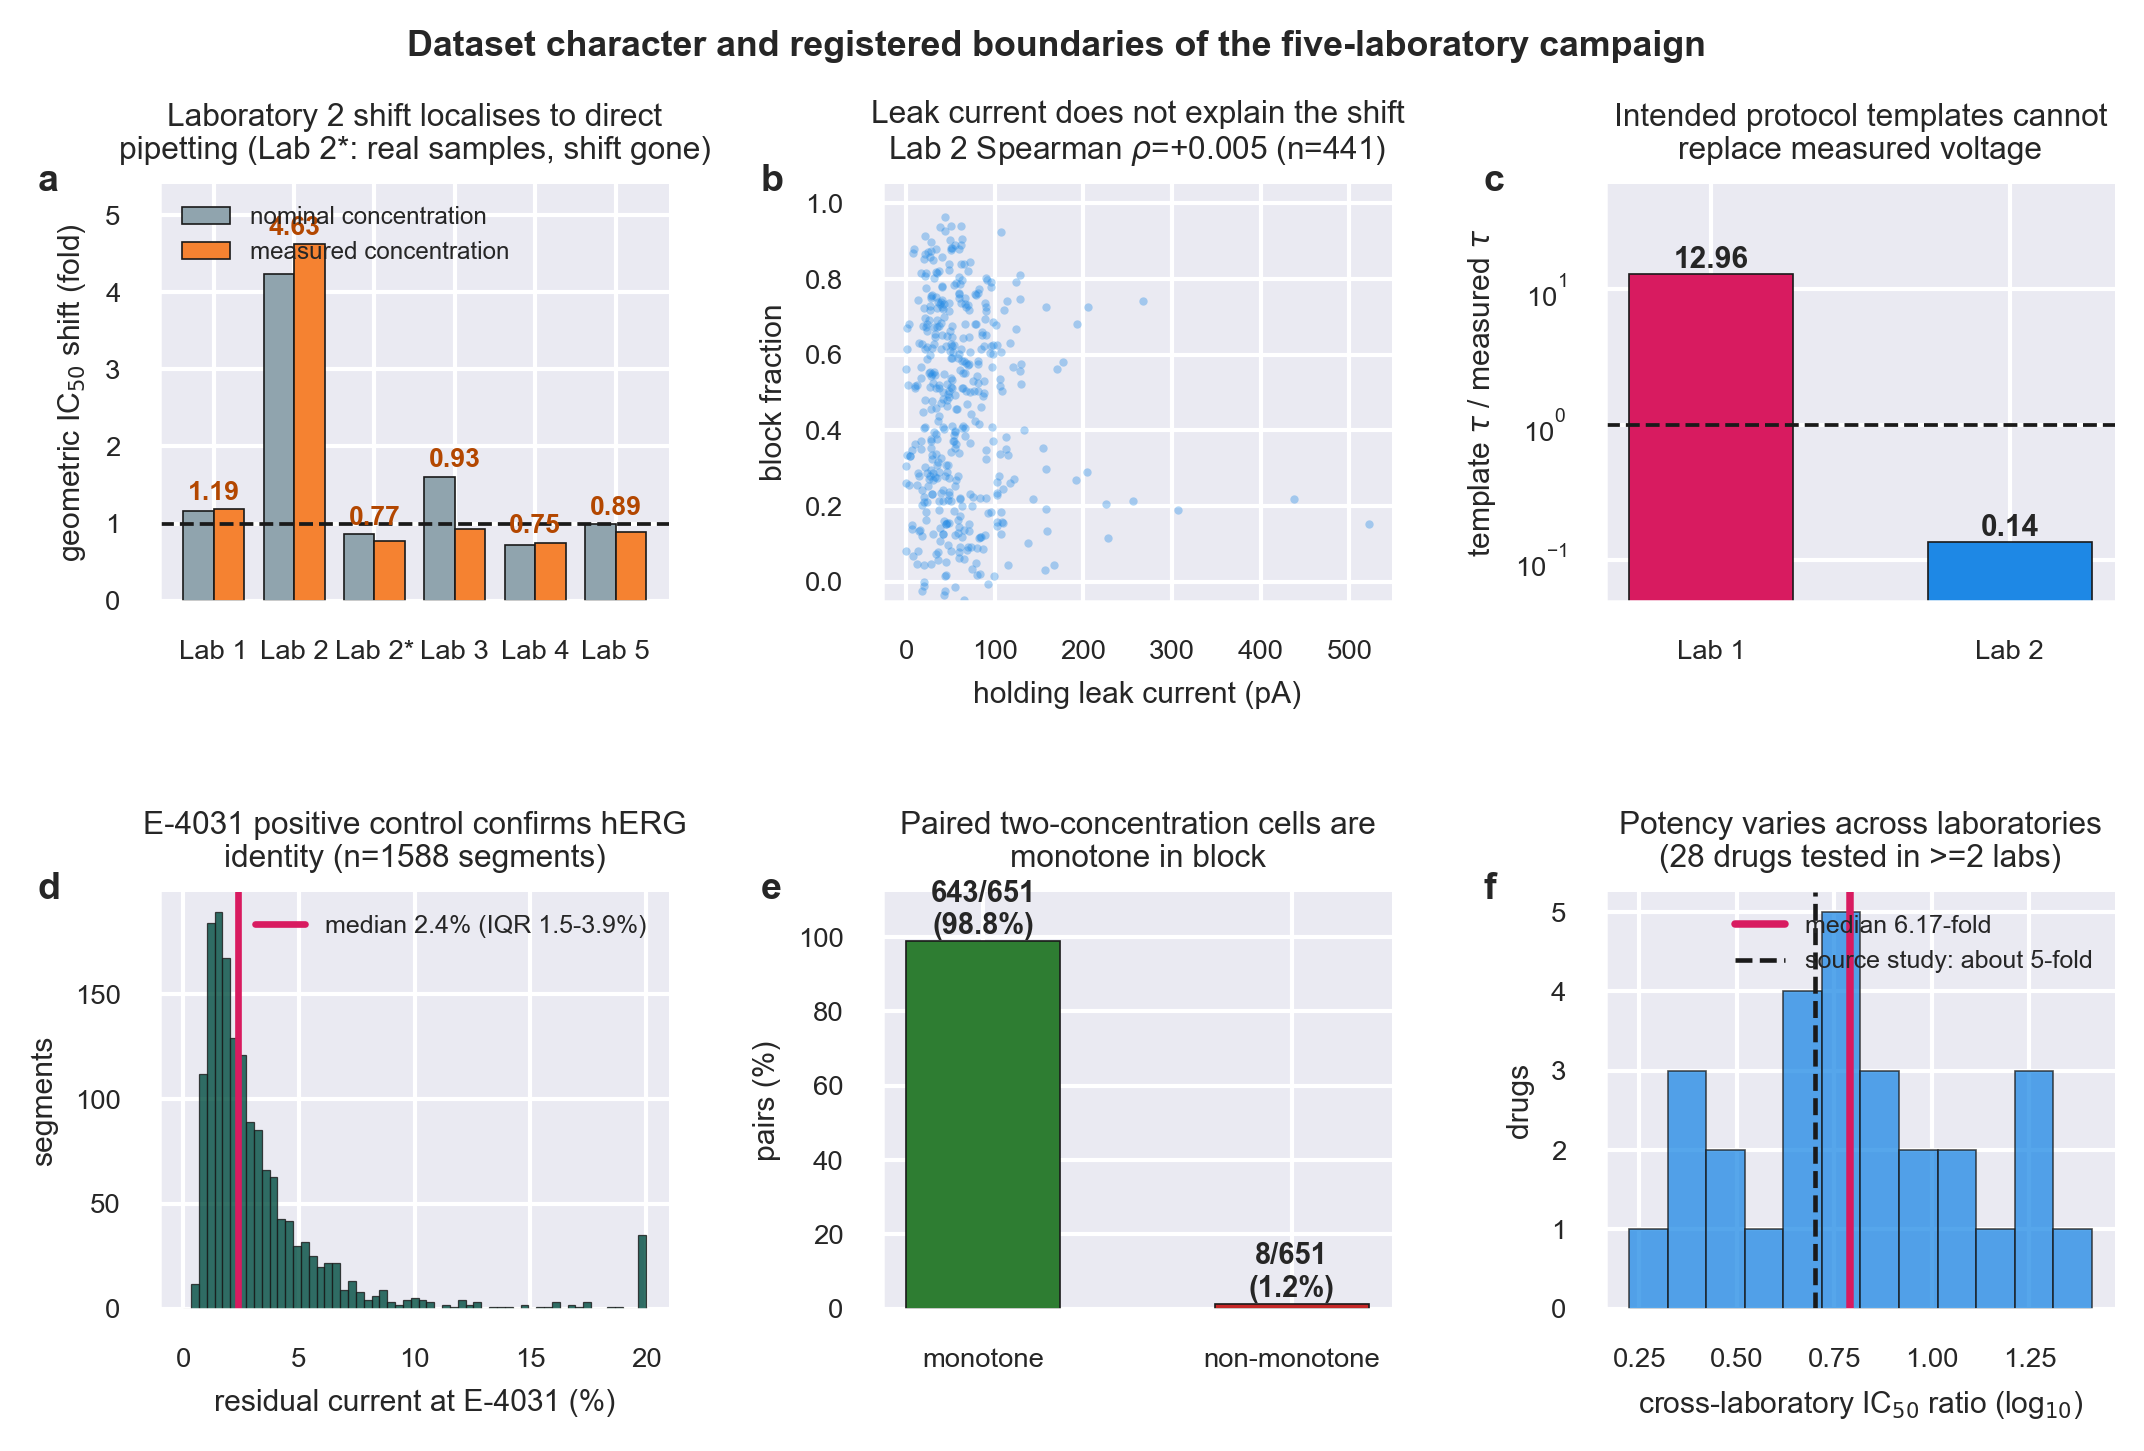
\includegraphics[width=\linewidth]{figS_fivelab_defects.png}
\caption{\textbf{Dataset character and registered boundaries of the
five-laboratory campaign.} (a) Per-laboratory geometric IC$_{50}$ shift with
nominal and measured concentrations; laboratory 2 assayed on real samples
(laboratory 2*) loses its shift (0.77). (b) Holding leak current versus block
fraction in laboratory 2 (Spearman $\rho=+0.006$, $n=441$). (c)
Template-voltage reconstruction returns control time constants 12.96-fold too
slow (laboratory 1) and 0.14-fold too fast (laboratory 2), so
intended-protocol templates cannot replace measured voltage. (d) E-4031
positive-control residuals (median 2.4\%, IQR 1.5--3.9\%, $n=1{,}588$
segments). (e) Paired two-concentration cells are monotone in block in 643 of
651 pairs (98.8\%). (f) Cross-laboratory IC$_{50}$ ratios (median 6.17-fold,
$n=28$ drugs; source-study expectation about five-fold).}
\label{fig:defects}
\end{figure}

\FloatBarrier
\section{Why Kir and K2P do not enter the verdict}

The verdict rule requires two scatters per group: a time constant and a
Boltzmann midpoint. Kir channels carry inward-rectifier currents whose
quasi-steady-state curves are rectification-dominated rather than S-shaped, so
no Boltzmann midpoint exists to scatter; a large fraction of Kir cells is
silent at the holding potential used by the recording protocol, which removes
the tail segments needed for deactivation fits. K2P channels are leak
channels: their currents are instantaneously open rectifiers without gated
S-shaped curves, and the two TASK-3 groups that had been carried in an earlier
66-group frame were removed as a grouping impurity. Both families remain in
the master table with their extracted quantities and flags; they simply have
no well-posed midpoint axis on which the verdict could run. Pure leak currents
are subtracted in every corpus by the same peak-minus-baseline construction.

\FloatBarrier
\section{Per-group verdict table}

\begin{longtable}{lllrrl}
\caption{Per-group conservation verdicts. Ratio (obs) is the raw scatter ratio; Ratio (shrunk) is the headline calibre (hierarchical partial pooling with profile-likelihood per-row uncertainties); Pass marks shrunk ratio above one. Groups with too few valid midpoint fits for shrinkage are marked n/a and do not enter the pass counts. $^{a}$Raw ratio off scale: bound-hit Boltzmann fits collapse the slope normalisation; calibre B removes exactly such fits.}\label{tab:verdictlong}\\
\toprule
Layer & Channel & Temp ($^\circ$C) & Ratio (obs) & Ratio (shrunk) & Pass \\
\midrule
\endfirsthead
\multicolumn{6}{l}{\footnotesize Table \ref{tab:verdictlong} (continued)}\\
\toprule
Layer & Channel & Temp ($^\circ$C) & Ratio (obs) & Ratio (shrunk) & Pass \\
\midrule
\endhead
\midrule\multicolumn{6}{r}{\footnotesize continued on next page}\\
\endfoot
\bottomrule
\endlastfoot
HCN activation & HCN1 & 15 & 8.25 & 8.03 & yes \\
HCN activation & HCN1 & 25 & 11.79 & 9.96 & yes \\
HCN activation & HCN2 & 25 & 14.29 & 13.49 & yes \\
HCN activation & HCN4 & 25 & 3.43 & 3.70 & yes \\
HCN activation & HCN4 & 35 & 5.07 & 5.31 & yes \\
\midrule
Kv activation & Kv1.1 & 15 & 9.39 & 3.09 & yes \\
Kv activation & Kv1.1 & 25 & 10.50 & 5.22 & yes \\
Kv activation & Kv1.1 & 35 & 4.39 & 4.43 & yes \\
Kv activation & Kv1.2 & 15 & 1.60 & 1.58 & yes \\
Kv activation & Kv1.2 & 25 & 1.90 & 1.86 & yes \\
Kv activation & Kv1.2 & 35 & 3.88 & 3.79 & yes \\
Kv activation & Kv1.3 & 15 & 22.61 & 4.51 & yes \\
Kv activation & Kv1.3 & 25 & 3.48 & 3.38 & yes \\
Kv activation & Kv1.3 & 35 & 3.59 & 3.52 & yes \\
Kv activation & Kv1.4 & 15 & 10.93 & 2.52 & yes \\
Kv activation & Kv1.4 & 25 & 3.43 & 3.27 & yes \\
Kv activation & Kv1.4 & 35 & 3.03 & 3.19 & yes \\
Kv activation & Kv1.5 & 15 & 2.89 & 1.33 & yes \\
Kv activation & Kv1.5 & 25 & 2.16 & 1.97 & yes \\
Kv activation & Kv1.5 & 35 & 11.71 & 2.85 & yes \\
Kv activation & Kv1.6 & 15 & 3.32 & 3.24 & yes \\
Kv activation & Kv1.6 & 25 & 2.97 & 2.92 & yes \\
Kv activation & Kv1.6 & 35 & 17.57 & 5.08 & yes \\
Kv activation & Kv1.7 & 15 & 15.85 & 2.31 & yes \\
Kv activation & Kv1.7 & 25 & 1.98 & 1.89 & yes \\
Kv activation & Kv1.7 & 35 & 3.55 & 2.87 & yes \\
Kv activation & Kv10.1 & 15 & 1.91 & 1.90 & yes \\
Kv activation & Kv10.1 & 25 & 3.95 & 3.48 & yes \\
Kv activation & Kv10.1 & 35 & 3.09 & 3.05 & yes \\
Kv activation & Kv10.1\_003 & 15 & 1.30 & 1.28 & yes \\
Kv activation & Kv10.1\_003 & 25 & 3.71 & 1.14 & yes \\
Kv activation & Kv10.1\_003 & 35 & 4.37 & 3.07 & yes \\
Kv activation & Kv10.2 & 35 & 10.57 & 4.13 & yes \\
Kv activation & Kv12.1 & 15 & 9.31 & 2.83 & yes \\
Kv activation & Kv12.1 & 25 & 3.57 & 2.94 & yes \\
Kv activation & Kv12.1 & 35 & 8.19 & 1.87 & yes \\
Kv activation & Kv12.3 & 15 & 8.46 & 6.33 & yes \\
Kv activation & Kv12.3 & 25 & 12.36 & 7.22 & yes \\
Kv activation & Kv12.3 & 35 & 15.25 & 8.02 & yes \\
Kv activation & Kv2.1 & 15 & 2.53 & 2.49 & yes \\
Kv activation & Kv2.1 & 25 & 2.78 & 2.66 & yes \\
Kv activation & Kv2.1 & 35 & 2.52 & 2.46 & yes \\
Kv activation & Kv2.1\_C1 & 25 & 2.61 & 2.43 & yes \\
Kv activation & Kv2.2 & 15 & 1.97 & 1.87 & yes \\
Kv activation & Kv2.2 & 25 & 2.98 & 1.79 & yes \\
Kv activation & Kv2.2 & 35 & 2.96 & 2.93 & yes \\
Kv activation & Kv3.1 & 15 & 1.65 & 1.32 & yes \\
Kv activation & Kv3.1 & 25 & 1.21 & 1.17 & yes \\
Kv activation & Kv3.1 & 35 & 1.38 & 1.67 & yes \\
Kv activation & Kv3.2 & 15 & 0.82 & 0.43 & no \\
Kv activation & Kv3.2 & 25 & 1.13 & 1.07 & yes \\
Kv activation & Kv3.2 & 35 & 1.82 & 1.64 & yes \\
Kv activation & Kv3.3 & 15 & 1.84 & 1.69 & yes \\
Kv activation & Kv3.3 & 25 & 1.58 & 1.57 & yes \\
Kv activation & Kv3.3 & 35 & 2.02 & 2.27 & yes \\
Kv activation & Kv3.4 & 15 & 1.85 & 1.82 & yes \\
Kv activation & Kv3.4 & 25 & 4.05 & 2.05 & yes \\
Kv activation & Kv3.4 & 35 & 3.14 & 1.50 & yes \\
Kv activation & Kv4.1 & 15 & 12.48 & 2.00 & yes \\
Kv activation & Kv4.1 & 25 & 9.24 & 3.56 & yes \\
Kv activation & Kv4.1 & 35 & 3.95 & 3.68 & yes \\
Kv activation & Kv4.2 & 15 & 11.10 & 2.48 & yes \\
Kv activation & Kv4.2 & 25 & 6.86 & 1.11 & yes \\
Kv activation & Kv4.2 & 35 & 5.91 & 1.79 & yes \\
Kv activation & Kv4.3 & 15 & 3.09 & 1.97 & yes \\
Kv activation & Kv4.3 & 25 & 2.37 & 2.31 & yes \\
Kv activation & Kv4.3 & 35 & 2.82 & 2.04 & yes \\
Kv activation & Kv7.1 & 15 & 4.62 & 3.63 & yes \\
Kv activation & Kv7.2D1 & 15 & 9.70 & 3.69 & yes \\
\midrule
Kv recovery & Kv1.1 & 15 & 4.20 & 3.59 & yes \\
Kv recovery & Kv1.1 & 25 & 6.14 & 4.65 & yes \\
Kv recovery & Kv1.1 & 35 & 4.25 & 3.95 & yes \\
Kv recovery & Kv1.2 & 15 & 2.57 & 2.73 & yes \\
Kv recovery & Kv1.2 & 25 & 4.13 & 3.78 & yes \\
Kv recovery & Kv1.2 & 35 & 3.32 & 6.12 & yes \\
Kv recovery & Kv1.3 & 15 & 5.44 & 4.59 & yes \\
Kv recovery & Kv1.3 & 25 & 2.27 & 2.35 & yes \\
Kv recovery & Kv1.3 & 35 & 1.85 & 2.15 & yes \\
Kv recovery & Kv1.4 & 15 & 2.33 & 2.01 & yes \\
Kv recovery & Kv1.4 & 25 & 1.56 & 1.28 & yes \\
Kv recovery & Kv1.4 & 35 & 2.37 & 1.84 & yes \\
Kv recovery & Kv1.5 & 15 & 1.21 & 1.24 & yes \\
Kv recovery & Kv1.5 & 25 & 3.06 & 2.68 & yes \\
Kv recovery & Kv1.5 & 35 & 2.66 & 2.09 & yes \\
Kv recovery & Kv1.6 & 15 & 6.35 & 4.17 & yes \\
Kv recovery & Kv1.6 & 25 & 6.40 & 5.06 & yes \\
Kv recovery & Kv1.6 & 35 & 5.16 & 4.62 & yes \\
Kv recovery & Kv1.7 & 15 & 1.34 & 1.00 & no \\
Kv recovery & Kv1.7 & 25 & 1.32 & 1.26 & yes \\
Kv recovery & Kv10.1 & 25 & 1.40 & 1.16 & yes \\
Kv recovery & Kv2.1 & 15 & 2.52 & 2.37 & yes \\
Kv recovery & Kv2.1 & 25 & 3.00 & 2.88 & yes \\
Kv recovery & Kv2.1 & 35 & 2.74 & 2.72 & yes \\
Kv recovery & Kv2.1\_C1 & 25 & 2.31 & 2.97 & yes \\
Kv recovery & Kv2.2 & 15 & 3.48 & 1.20 & yes \\
Kv recovery & Kv2.2 & 25 & 5.96 & 3.04 & yes \\
Kv recovery & Kv2.2 & 35 & 1.57 & 1.77 & yes \\
Kv recovery & Kv3.1 & 15 & 0.98 & 0.91 & no \\
Kv recovery & Kv3.1 & 25 & 1.97 & 1.99 & yes \\
Kv recovery & Kv3.1 & 35 & 2.41 & 2.43 & yes \\
Kv recovery & Kv3.2 & 15 & 2.19 & 1.86 & yes \\
Kv recovery & Kv3.2 & 25 & 1.28 & 1.26 & yes \\
Kv recovery & Kv3.3 & 15 & 1.98 & 2.50 & yes \\
Kv recovery & Kv3.3 & 25 & 1.92 & 2.14 & yes \\
Kv recovery & Kv3.3 & 35 & 2.44 & 2.14 & yes \\
Kv recovery & Kv3.4 & 15 & 0.80 & 0.86 & no \\
Kv recovery & Kv3.4 & 25 & 1.35 & 1.43 & yes \\
Kv recovery & Kv4.1 & 15 & 1.20 & 1.22 & yes \\
Kv recovery & Kv4.1 & 25 & 1.49 & 2.35 & yes \\
Kv recovery & Kv4.3 & 15 & 1.36 & 1.05 & yes \\
Kv recovery & Kv4.3 & 25 & 1.23 & 1.40 & yes \\
\midrule
Kv deactivation & Kv1.1 & 15 & 6.99 & 3.77 & yes \\
Kv deactivation & Kv1.1 & 25 & 6.62 & 3.32 & yes \\
Kv deactivation & Kv1.1 & 35 & 3.96 & 3.10 & yes \\
Kv deactivation & Kv1.2 & 15 & 3.35 & 3.35 & yes \\
Kv deactivation & Kv1.2 & 25 & 2.85 & 2.86 & yes \\
Kv deactivation & Kv1.2 & 35 & 3.83 & 2.95 & yes \\
Kv deactivation & Kv1.3 & 15 & 13.75 & 4.50 & yes \\
Kv deactivation & Kv1.3 & 25 & 2.99 & 2.93 & yes \\
Kv deactivation & Kv1.3 & 35 & 3.07 & 3.06 & yes \\
Kv deactivation & Kv1.4 & 15 & 2.67 & 0.61 & no \\
Kv deactivation & Kv1.4 & 25 & 0.97 & 0.83 & no \\
Kv deactivation & Kv1.5 & 15 & 4.63 & 2.14 & yes \\
Kv deactivation & Kv1.5 & 25 & 1.93 & 2.10 & yes \\
Kv deactivation & Kv1.5 & 35 & 10.64 & 2.59 & yes \\
Kv deactivation & Kv1.6 & 15 & 2.30 & 2.66 & yes \\
Kv deactivation & Kv1.6 & 25 & 2.77 & 2.85 & yes \\
Kv deactivation & Kv1.6 & 35 & 12.53 & 3.28 & yes \\
Kv deactivation & Kv1.7 & 15 & 3.39 & n/a & n/a \\
Kv deactivation & Kv1.7 & 25 & 1.02 & n/a & n/a \\
Kv deactivation & Kv10.1 & 15 & 5.11 & 6.18 & yes \\
Kv deactivation & Kv10.1 & 25 & 5.09 & 4.55 & yes \\
Kv deactivation & Kv10.1 & 35 & 1.24 & n/a & n/a \\
Kv deactivation & Kv10.1\_003 & 15 & 1.31 & 1.33 & yes \\
Kv deactivation & Kv10.1\_003 & 25 & 16.69 & 5.34 & yes \\
Kv deactivation & Kv10.1\_003 & 35 & 3.26 & n/a & n/a \\
Kv deactivation & Kv12.1 & 15 & 5.64 & 4.93 & yes \\
Kv deactivation & Kv12.1 & 25 & 2.94 & 2.49 & yes \\
Kv deactivation & Kv12.1 & 35 & 15.57 & 4.80 & yes \\
Kv deactivation & Kv12.3 & 25 & 12.05 & 9.66 & yes \\
Kv deactivation & Kv12.3 & 35 & 11.67 & n/a & n/a \\
Kv deactivation & Kv2.1 & 15 & 2.50 & 2.60 & yes \\
Kv deactivation & Kv2.1 & 25 & 2.90 & 2.80 & yes \\
Kv deactivation & Kv2.1 & 35 & 2.02 & 2.46 & yes \\
Kv deactivation & Kv2.1\_C1 & 25 & 3.36 & 3.14 & yes \\
Kv deactivation & Kv2.2 & 15 & 1.82 & 1.68 & yes \\
Kv deactivation & Kv2.2 & 25 & 2.50 & 1.56 & yes \\
Kv deactivation & Kv2.2 & 35 & 3.75 & 4.19 & yes \\
Kv deactivation & Kv3.1 & 15 & 2.74 & 2.34 & yes \\
Kv deactivation & Kv3.1 & 25 & 3.55 & 3.81 & yes \\
Kv deactivation & Kv3.1 & 35 & 1.65 & 1.94 & yes \\
Kv deactivation & Kv3.2 & 15 & 2.44 & 1.33 & yes \\
Kv deactivation & Kv3.2 & 25 & 3.56 & 3.42 & yes \\
Kv deactivation & Kv3.2 & 35 & 4.27 & 4.45 & yes \\
Kv deactivation & Kv3.3 & 15 & 3.49 & 3.33 & yes \\
Kv deactivation & Kv3.3 & 25 & 3.23 & 3.41 & yes \\
Kv deactivation & Kv3.3 & 35 & 0.92 & 0.88 & no \\
Kv deactivation & Kv3.4 & 15 & 1.30 & 1.15 & yes \\
Kv deactivation & Kv3.4 & 25 & 4.47 & 2.33 & yes \\
Kv deactivation & Kv3.4 & 35 & 3.38 & 2.25 & yes \\
Kv deactivation & Kv4.1 & 15 & 5.41 & 0.89 & no \\
Kv deactivation & Kv4.1 & 25 & 3.67 & n/a & n/a \\
Kv deactivation & Kv4.3 & 15 & 1.63 & 1.05 & yes \\
Kv deactivation & Kv4.3 & 25 & 0.69 & n/a & n/a \\
Kv deactivation & Kv7.1 & 15 & 0.56 & 0.56 & no \\
Kv deactivation & Kv7.2D1 & 15 & 2.93 & 1.94 & yes \\
\midrule
Kv inactivation & Kv1.1 & 15 & 10.04 & n/a & n/a \\
Kv inactivation & Kv1.1 & 25 & 5.96 & 2.97 & yes \\
Kv inactivation & Kv1.1 & 35 & 3.38 & 3.24 & yes \\
Kv inactivation & Kv1.2 & 25 & 2.05 & 1.98 & yes \\
Kv inactivation & Kv1.2 & 35 & 2.27 & 2.22 & yes \\
Kv inactivation & Kv1.3 & 15 & 11.83 & 2.42 & yes \\
Kv inactivation & Kv1.3 & 25 & 1.36 & 1.33 & yes \\
Kv inactivation & Kv1.3 & 35 & 1.21 & 1.18 & yes \\
Kv inactivation & Kv1.4 & 15 & 8.66 & 1.89 & yes \\
Kv inactivation & Kv1.4 & 25 & 2.40 & 2.18 & yes \\
Kv inactivation & Kv1.4 & 35 & 2.78 & 2.89 & yes \\
Kv inactivation & Kv1.5 & 15 & 2.19 & n/a & n/a \\
Kv inactivation & Kv1.5 & 25 & 1.15 & 1.05 & yes \\
Kv inactivation & Kv1.5 & 35 & 5.08 & 1.24 & yes \\
Kv inactivation & Kv1.6 & 15 & 2.05 & n/a & n/a \\
Kv inactivation & Kv1.6 & 25 & 2.48 & 2.45 & yes \\
Kv inactivation & Kv1.6 & 35 & 15.77 & 4.02 & yes \\
Kv inactivation & Kv1.7 & 15 & 8.74 & 1.07 & yes \\
Kv inactivation & Kv1.7 & 25 & 1.53 & 1.52 & yes \\
Kv inactivation & Kv1.7 & 35 & 3.16 & 3.71 & yes \\
Kv inactivation & Kv10.1\_003 & 25 & 4.37 & n/a & n/a \\
Kv inactivation & Kv12.1 & 35 & 25.05 & n/a & n/a \\
Kv inactivation & Kv2.1 & 15 & off-scale$^{a}$ & n/a & n/a \\
Kv inactivation & Kv2.1 & 25 & 1.25 & 1.19 & yes \\
Kv inactivation & Kv2.1 & 35 & 1.33 & 1.30 & yes \\
Kv inactivation & Kv2.1\_C1 & 25 & 0.98 & 0.91 & no \\
Kv inactivation & Kv2.2 & 15 & 6.66 & n/a & n/a \\
Kv inactivation & Kv2.2 & 25 & 1.07 & 0.64 & no \\
Kv inactivation & Kv2.2 & 35 & 1.45 & 1.45 & yes \\
Kv inactivation & Kv3.1 & 25 & 0.81 & n/a & n/a \\
Kv inactivation & Kv3.1 & 35 & 0.96 & 0.85 & no \\
Kv inactivation & Kv3.2 & 25 & 0.77 & 0.73 & no \\
Kv inactivation & Kv3.2 & 35 & 1.07 & 1.01 & yes \\
Kv inactivation & Kv3.3 & 15 & 1.72 & 1.02 & yes \\
Kv inactivation & Kv3.3 & 25 & 0.91 & 0.90 & no \\
Kv inactivation & Kv3.3 & 35 & 1.01 & 1.00 & yes \\
Kv inactivation & Kv3.4 & 15 & 0.50 & 0.50 & no \\
Kv inactivation & Kv3.4 & 25 & 1.86 & 0.94 & no \\
Kv inactivation & Kv3.4 & 35 & 1.10 & 1.12 & yes \\
Kv inactivation & Kv4.1 & 15 & 10.02 & 1.61 & yes \\
Kv inactivation & Kv4.1 & 25 & 7.35 & 2.96 & yes \\
Kv inactivation & Kv4.2 & 15 & 11.96 & n/a & n/a \\
Kv inactivation & Kv4.3 & 15 & 2.90 & 1.85 & yes \\
Kv inactivation & Kv4.3 & 25 & 3.20 & 3.08 & yes \\
Kv inactivation & Kv4.3 & 35 & 0.86 & n/a & n/a \\
Kv inactivation & TASK3 & 35 & 2.42 & n/a & n/a \\
\end{longtable}


\FloatBarrier
\section{Host-model integration and CiPA scoring}

Table~\ref{tab:hostchecks} gives the host-level acceptance checks J1--J6 for
the O'Hara--Rudy composite with measured-table $I_{\mathrm{Kr}}$ and
$I_{\mathrm{Ks}}$. Table~\ref{tab:cipaarms} gives the per-arm CiPA scoring on
the 24 shared risk-labelled drugs.

\begin{table}[htbp]\centering\small
\caption{Host-level checks J1--J6 for the O'Hara--Rudy composite with
measured-table $I_{\mathrm{Kr}}$ and $I_{\mathrm{Ks}}$.}
\label{tab:hostchecks}
\begin{tabular}{@{}p{2.2cm}p{4.4cm}p{5.6cm}p{3.4cm}@{}}
\toprule
check & content & measured & band \\
\midrule
J1 & last-10-beat APD90 range & 0.005\,ms & $<0.5$\,ms \\
J2 & APD90 / APA / RMP / qNet & 251.206\,ms ($\Delta$0.36\%) / 128.51\,mV / $-87.99$\,mV / 0.056 & APD90 $\pm2$\%; APA 124.4--130; RMP $-95$ to $-85$ \\
J3a & $I_{\mathrm{Kr}}$-only swap, trace agreement & $1.1\times10^{-5}$ & $\le1$\% \\
J3b & $I_{\mathrm{Ks}}$-only swap & APD90 255.77; APA 127.94; RMP $-88.00$; qNet 0.0717 & all in band \\
J3c & N-arm registration & APA saturated; $\Delta$APA $=3.1\times10^{-5}$\,mV at $G\times16$ & expected-failure signature \\
J4 & upstroke d$V$/d$t_{\max}$ & 240.7 vs.\ 236.6\,V/s (1.017) & 50--500\,V/s \\
J5 & rate dependence & monotone shortening; 1:1 capture; max difference 2.5\,ms & monotone + capture \\
J6 & peak-current ratios & $I_{\mathrm{Kr}}$ 2.06; $I_{\mathrm{Ks}}$ 1.52; $I_{\mathrm{Na}}$ 0.997; $I_{\mathrm{CaL}}$ 0.979; $I_{\mathrm{NaL}}$ 1.009; $I_{\mathrm{to}}$ 1.002; $I_{\mathrm{K1}}$ 1.004 & all in 0.2--5 \\
\bottomrule
\end{tabular}
\end{table}

\begin{table}[htbp]\centering\small
\caption{CiPA scoring arms on the 24 shared drugs.}
\begin{tabular}{@{}llcc@{}}
\toprule
arm & model & V1 $\rho$ & V2 AUC \\
\midrule
B1 & official Markov 9-state + static Hill & $-0.523$ & 0.833 \\
B2s & measured-table + static binding & $-0.506$ & 0.833 \\
B2 & measured-table + dynamic binding & $-0.547$ ($p=0.0057$) & 0.857 \\
\bottomrule
\end{tabular}
\label{tab:cipaarms}
\end{table}

The cross-laboratory carry test of the main text substitutes the Channelpedia
population hERG time-constant table for the sealed single-cell kinetics and
scores the prediction of CiPA screening traces cell by cell under the frozen
acceptance criteria. The population-table model passes 67 of 68 cells
(laboratory 3: 20/20; laboratory 4: 16/16; laboratory 5: 29/32; manual: 3/3),
against 65 of 68 for the sealed-table model, and no cell moves from pass to
fail. The two rescued cells sit in laboratory 5, whose recordings carry the
largest voltage-clamp uncertainty of the panel.

\FloatBarrier
\section{Data and code}

All source datasets are public; their repository identifiers are listed in
Table 1 of the main text. The unified master table (487,940 rows including the
356 reference-layer rows), the extraction and verdict code, the figure scripts
and the per-layer verdict tables are deposited at Zenodo
(\url{https://doi.org/10.5281/zenodo.23042212}) and mirrored at GitHub
(\url{https://github.com/lihuanlz/alpha-ion-channel-models}). The earlier
four-channel preprint is at Research Square
(\url{https://doi.org/10.21203/rs.3.rs-11218939/v1}).

\end{document}
